\chapter{Moving Obstacle Avoidance}

\section{Problem Formulation}
% COLLISION AVOIDANCE FIGURE
\begin{figure}[!h]
	\centering
	\includegraphics[width=\textwidth]{../figure/obstacleAvoidance/obstacleAvoidance.pdf}
	\caption{Problem description of collision avoidance on a road with only two lanes.}
	\label{fig:obstacleAvoidance}
\end{figure}
% BICYCLE MODEL
\begin{figure}[!h]
	\centering
	\includegraphics[width=0.80\textwidth]{../figure/car_model.pdf}
	\caption{Bicycle model of a car, (adapted from \cite{siciliano}).}
	\label{fig:car_model}
\end{figure}
\section{Design of Adaptive MPC}
% FLOWCHART
\begin{figure}[!h]
	\centering
	\includegraphics[width=\textwidth]{../figure/flowchart/flowchart.pdf}
	\caption{Behaviour planning conditional flowchart.}
	\label{fig:flowchart}
\end{figure}
% FIGURE CONSTRAINT
\begin{figure}[!h]
	\centering
	\includegraphics[width=\textwidth]{../figure/constraint/constraint.pdf}
	\caption{Constraints in the case of left overtaking.}
	\label{fig:constraint}
\end{figure}


\section{Simulation Results}
% ONE MOVING OBSTACLE
\begin{figure}[h!]
	\centering
	\begin{minipage}[t]{\textwidth}
		\includegraphics[width=\textwidth]{../figure/one_obstacle_right_overtaking/overtaking_start.pdf}
	\end{minipage}
	\begin{minipage}[t]{\textwidth}
		\includegraphics[width=\textwidth]{../figure/one_obstacle_right_overtaking/overtaking_middle.pdf}
	\end{minipage}
	\begin{minipage}[t]{\textwidth}
		\includegraphics[width=\textwidth]{../figure/one_obstacle_right_overtaking/overtaking_middle_end.pdf}
	\end{minipage}
	\begin{minipage}[t]{\textwidth}
		\includegraphics[width=\textwidth]{../figure/one_obstacle_right_overtaking/overtaking_end.pdf}
	\end{minipage}
	\caption{Simulation of right overtaking with one moving obstacle that moves in the same direction as the vehicle.}
	\label{fig:obstacleAvoidance_one_obstacle}
\end{figure}
% ALGORITHM FOR RIGHT OVERTAKING OF ONE MOVING OBSTACLE
\begin{algorithm}%[b]
	\caption{Right Overtaking if an obstacle is detected}
	\small
	\begin{algorithmic}[1]
		\Function{RightOvertaking}{car, obstacle, road}
		\State $x_\text{min} \gets \text{car}X $,  $x_\text{max} \gets +\infty$;
		\State obsYrr = obstacle.RearRightSafeY;
		\State obsXrr = obstacle.RearRightSafeX;
		\If{ATLASCAR2 is behind the obstacle} 
		\If{ATLASCAR2 is in the adjacent lane}
		\State $cS \gets 0$; $cI \gets \text{obsYrr}$;
		\Else
		\State $cS \gets \text{tan}(\text{atan2}(\frac{\text{obsYrr}-\text{ carY}}{\text{obsXrr}-\text{carX}},1))$;
		\State $cI \gets \text{obsYrr}-cS*\text{obsXrr}$;
		\EndIf
		\Else
		\If{ATLASCAR2 is parallel to the obstacle}
		\State $cS \gets 0$; $cI \gets \text{obsYrr}$;
		\Else
		\State $cS \gets 0$; $cI \gets W/2$;
		\EndIf
		\EndIf
		\State \Return $x_\text{min}$, $x_\text{max}$, $cI$, $cS$
		\EndFunction
	\end{algorithmic}
	\label{alg:rightOvertaking}
\end{algorithm}
% OVERALL SCHEME ONE MOVING OBSTACLE
\begin{figure}[!h]
	\centering
	\includegraphics[width=\textwidth]{../figure/MovingObstacleAvoidance.pdf}
	\caption{Overall procedure scheme moving obstacle avoidance.}
	\label{fig:MovingObstacleAvoidance}
\end{figure}
% MULTIPLE MOVING OBSTACLE
\begin{figure}[!h]
	\centering
	\begin{minipage}[t]{\textwidth}
		\includegraphics[width=\textwidth]{./figure/random_N_obstacles/overtaking_random_2.pdf}
	\end{minipage}
	\begin{minipage}[t]{\textwidth}
		\includegraphics[width=\textwidth]{./figure/random_N_obstacles/overtaking_random.pdf}
	\end{minipage}
	\begin{minipage}[t]{\textwidth}
		\includegraphics[width=\textwidth]{./figure/random_N_obstacles/overtaking_random_1.pdf}
	\end{minipage}
	\caption{Simulations of overtaking with $N = 2,3,4$ moving obstacles that drive in the opposite direction with respect to the ATLASCAR2.}
	\label{fig:obstacleAvoidance_random}
\end{figure}

% BRAKING THREE OBSTACLE
\begin{figure}[!h]
	\centering
	\begin{minipage}[t]{\textwidth}
		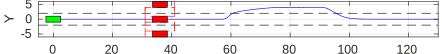
\includegraphics[width=\textwidth]{./figure/three_obstacles_no_overtaking/braking_0.pdf}
	\end{minipage}
	\begin{minipage}[t]{\textwidth}
		\includegraphics[width=\textwidth]{./figure/three_obstacles_no_overtaking/braking_1.pdf}
	\end{minipage}
	\begin{minipage}[t]{\textwidth}
		\includegraphics[width=\textwidth]{./figure/three_obstacles_no_overtaking/braking_2.pdf}
	\end{minipage}
	\begin{minipage}[t]{\textwidth}
		\includegraphics[width=\textwidth]{./figure/three_obstacles_no_overtaking/braking_3.pdf}
	\end{minipage}
	\begin{minipage}[t]{\textwidth}
		\includegraphics[width=\textwidth]{./figure/three_obstacles_no_overtaking/braking_4.pdf}
	\end{minipage}
	\begin{minipage}[t]{\textwidth}
		\includegraphics[width=\textwidth]{./figure/three_obstacles_no_overtaking/braking_5.pdf}
	\end{minipage}
	\begin{minipage}[t]{\textwidth}
		\includegraphics[width=\textwidth]{./figure/three_obstacles_no_overtaking/braking_6.pdf}
	\end{minipage}
	\caption{Simulation of braking and overtaking obstacles.}
	\label{fig:braking}
\end{figure}
% RESULTS BRAKING THREE OBSTACLES
\begin{figure}[!t] %vs changes to t instead of b
	\begin{minipage}[t]{0.5\textwidth}
		\includegraphics[width=\textwidth]{./figure/three_obstacles_no_overtaking/VelocityVsTime.pdf}
		\vspace{-17pt}
		\subcaption{}\label{fig:velocity_braking}
	\end{minipage}
	\begin{minipage}[t]{0.5\textwidth}
		\includegraphics[width=\textwidth]{./figure/three_obstacles_no_overtaking/ThrottleVsTime.pdf}
		\vspace{-17pt}
		\subcaption{}\label{fig:throttle_braking}
	\end{minipage}
	\begin{minipage}[t]{0.5\textwidth}
		\includegraphics[width=\textwidth]{./figure/three_obstacles_no_overtaking/SteeringAngleVsTime.pdf}
		\vspace{-17pt}
		\subcaption{}\label{fig:delta_braking}
	\end{minipage}
	\begin{minipage}[t]{0.5\textwidth}
		\includegraphics[width=\textwidth]{./figure/three_obstacles_no_overtaking/HeadingAngleVsTime.pdf}
		\vspace{-17pt}
		\subcaption{}\label{fig:theta_braking}
	\end{minipage}
	\caption{Time signals of the ATLASCAR2 in the simulation of braking and overtaking in the situation illustrated in Fig. \ref{fig:braking}.}
	\label{fig:components}
\end{figure}
